\documentclass[a4paper,12pt]{article}
\usepackage{amsmath}
\usepackage{amsfonts}
\usepackage{amssymb}
\usepackage{geometry}
\usepackage{fancyhdr}
\usepackage{multicol}
\usepackage{graphicx}

% Page layout
\geometry{margin=1in}

% Header and footer
\pagestyle{fancy}
\fancyhf{}
\fancyhead[L]{Examen Estructuras Algebraicas}
\fancyhead[C]{4º MAIS}
\fancyhead[R]{Antonio Cabrera Landín}
\fancyfoot[C]{\thepage}

\begin{document}

\begin{center}
    \textbf{\Large Estructuras 2024/25. Examen parcial} \\
    \textbf{Profesor: Georgy Nuzhdin. Fecha: 05.11.2024} \\
\end{center}

\section*{Teoremas}
\begin{enumerate}
    \item (0.3) En níngun grupo puede haber dos elementos neutros distintos.
    \begin{equation*}
       \begin{split}
            & \text{Supongamos que existen dos nuetros } e_1, e_2 \in G \text{, tal que } e_{1} \neq e_{2}\\
            & \begin{cases}
                a \cdot e_{1} = a\\
                a \cdot e_{2} = a
            \end{cases} \implies a \cdot e_{1} = a \cdot e_{2} \iff a^{-1}ae_{1} = a^{-1}ae_{2} \iff e_{1} = e_{2}\\
            & \text{Contradicción: } e_{1} \neq e_{2} \text{ y } e_{1} = e_{2}
       \end{split} 
    \end{equation*}

    \item (0.5) Cualquier grupo de orden primo es cíclico.
    
    Sea $p$ el orden del grupo:
    \begin{itemize}
        \item Si el orden del grupo es primo, sus elementos deberán tener orden 1 o $p$
        \item El único elemento de orden 1 es el nuetro y solo puede haber uno por grupo.
        \item Por lo tanto, todos los elementos menos el neutro tienen orden igual a $p$.
        \item Como el grupo tiene generadores, se trata de un grupo cíclico
    \end{itemize}

    \pagebreak

    \item (0.7) Cualquier grupo es isomorfo a un subgrupo de algún grupo simétrico.

    Consideremos la acción $\varphi_g(x)=gx$ con $g \in G$ y $x \in G$. Sabemos que la acción de un elemento es una función biyectiva.

    Definamos ahora $\phi(g)=\varphi_g$, este isomorfismo formará el grupo de las biyecciones (subgrupo simétrico)

    Vamos a demostrar que $\{\phi(g):g \in G\}$ con la operación composición de funciones es un subgrupo:

    \begin{itemize}
        \item Cumple con la asociativa ya que la composición de funciones es asociativa
        \item El elemento neutro es $\varphi_e$:
        $$
        (\varphi_{e} \circ \varphi_{a})(x) = eax = ax = \varphi_a(x) \implies \varphi_{e} \circ \varphi_{a} = \varphi_{a} \implies \varphi_e \text{ es el neutro}
        $$
        \item El inverso de $\varphi_a$ es $\varphi_{a^{-1}}$
        $$
        (\varphi_a \circ \varphi_{a^{-1}})(x) = aa^{-1}x = ex = \varphi_e(x) \implies \varphi_a \circ \varphi_{a^{-1}} = \varphi_e \implies (\varphi_a)^{-1} = \varphi_{a^{-1}}  
        $$
    \end{itemize}

    Ahora tenemos que demostrar que $\phi(g)$ es un isomorfismo de $G$, es decir, un homomorfismo biyectivo. Primero veremos que es un homomorfismo:
    $$
    \phi (ab) = \varphi_{ab} = abx = \varphi_a \circ \varphi_b = \phi(a) \circ \phi(b) \implies \phi \text{ es un homomorfismo}
    $$

    Falta comprobar que es biyectivo:
    \begin{itemize}
        \item Suprayectivo: La preimagen de $\varphi_a$ siempre es $a$
        \item Inyectivo:
        \begin{equation*}
            \begin{split}
                & \text{Supongamos que } \phi(a) = \phi(b) \text{ con } a\neq b\\
                & \phi (a) = \varphi_a = \varphi_b = \phi(b)\\
                & \varphi_a(x) = ax = \varphi_b(x) = bx \iff ax = bx \iff a = b\\
                & \text{Contradicción: } a\neq b \text{ y } a=b \text{, por lo tanto es biyectivo}
            \end{split} 
        \end{equation*}
    \end{itemize}

        Como conclusión, efectivamente cualquier grupo es isomorfo a un subgrupo de algún simétrico


    \item (0.7) Las clases laterales izquierdas o coinciden o no tienen intersección.
        \begin{equation*}
            \begin{split}
                & \text{Supongamos } a,b \in G \text{ tal que } x \in aH \text{ y } x \in bH \text{ con } a\neq b\\
                & \begin{cases}
                    x \in aH \implies x = ah_{1}\\
                    x \in bH \implies x = bh_{2}
                \end{cases} \implies ah_{1} = bh_{2} \iff ah_{1}(h_{1})^{-1} = bh_{2}(h_{1})^{-1} \iff\\
            & \iff a = bh_{3} \implies a \in bH\\
            & \forall a_1 \in aH \implies a_{1} = ah = bh_{3}h \in bH \implies aH = bH\\
            & \text{Por lo tanto, si $x$ comparte clases laterales, estás coinciden}
            \end{split} 
        \end{equation*}

        \pagebreak
    
    \item (1.0) $G / Kerf \cong Imf(f)$, siendo $f:G\to G'$ un homomorfismo.

    Primero, llamaremos $H = Kerf$

    La proyección $\pi(g)= gH$ asocia a cada elemento una clase lateral. Pero todas las imágenes de elementos del grupo $G$ son equivalentes "módulo" clase lateral. En concreto, los elementos que pasan al neutro $\pi (g) = eH = H$ son precisamente los elementos del subgrupo $H$.

    Definamos ahora el homomorfismo $\bar{f}$ tal que $\bar{f}(gH)=f(g)$. De esta manera, a la clase lateral del elemento $g$ le corresponde la imagen de $g$ por el homomorfismo original $f$.

    \begin{itemize}
        \item Necesitamos comprobar que es una definición correcta, es decir, no depende del representante de la clase lateral $g$.
        \begin{equation*}
            \begin{split} 
                & \text{Sea } g_{1}H = g_{2}H \implies g_2 = g_{1}h, \; h \in H \implies\\
                & \implies f(g_{2})=f(g_{1})*f(h)=f(g_{1})*e \text{, ya que } h \in H \subset Kerf
            \end{split}
        \end{equation*}

        \item También hay que tener en cuenta que $gH * hH = g(hH) * H = (gh)H * H = ghH$ porque $H$ es normal.
    \end{itemize}
    
    Vamos a demostrar que $\bar{f}$ es un isomorfismo (homomorfismo biyectivo)
    
    \begin{itemize}

        \item $\bar{f}$ es un homomorfismo
        $$
        \bar{f}(gH * hH) = \bar{f}(ghH) = f(gh) = f(g)*f(h)
        $$

        \item $\bar{f}$ es inyectivo. Hay que demostrar que $\bar{f}(aH) = \bar{f}(bH) \implies aH = bH$
        \begin{equation*}
            \begin{split}
                & \bar{f}(aH) = \bar{f}(bH) \iff f(a) = f(b) \iff f(ab^{-1}) = f(bb^{-1}) \iff f(ab^{-1}) = e \iff\\
                & \iff ab^{-1} \in Kerf = H \iff ab^{-1} \in eH \iff a \in Hb = bH \implies aH = bH  
            \end{split}
        \end{equation*}

    \item $\bar{f}$ es suprayectivo, ya que $Im \bar{f} = Imf$ 
    \end{itemize}
\end{enumerate}

\pagebreak

\section*{Ejercicios}

\begin{enumerate}
    \item Averigua si es semigrupo, monoide o grupo el conjunto de todos los subconjuntos del conjunto $A$ con la operación:

    \begin{enumerate}
        \item (0.2) La unión ($\cup$)

        \begin{itemize}
            \item Se cumple la propiedad asociativa ya que $(A\cup B)\cup C = A \cup (B \cup C)$
            \item El neutro sería el conjunto vacío $\emptyset$
            \item No existe el inverso de ningún elemento ya que la unión nunca va a disminuir el cardinal de los conjuntos originales (la unión de conjuntos no vacíos nunca tiene cardinal nulo)
                $$|A\cup B| \ge |A|$$
        \end{itemize}

        \item (0.4) $A*B = (A \cup B) \setminus (A \cap B)$

        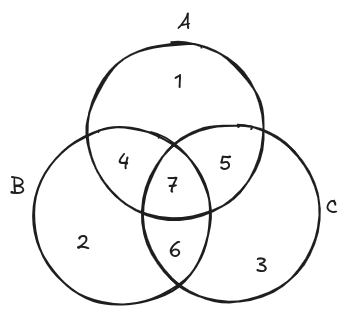
\includegraphics[scale=0.4]{./diagramas.png} 

        \begin{itemize}
            \item Cumple la asociativa:
                \begin{equation*}
                    \begin{split}
                        & A*B = (A\cup B) \setminus (A \cap B) = 1, 2, 5, 6\\
                        & B*C= (B\cup C) \setminus (B \cap C) = 2, 3, 4, 5\\
                        & (A*B)*C = (((A\cup B) \setminus (A \cap B)) \cup C) \setminus (((A \cup B) \setminus (A \cap B)) \cap C) =\\
                        & = ((1,2,5,6) \cup (3,5,6,7)) \setminus ((1,2,5,6) \cap (3,5,6,7)) = \\
                        & = (1,2,3,5,6,7) \setminus (5,6) = (1,2,3,7) \\
                        & A * (B*C) = (A \cup ((B \cup C)\setminus(B \cap C))) \setminus (A \cap ((B \cup C)\setminus(B \cap C))) =\\
                        & = ((1,4,5,7) \cup (2,3,4,5)) \setminus ((1,4,5,7)\cap (2,3,4,5)) =\\
                        & = (1,2,3,4,5,7) \setminus (4,5) = (1,2,3,7)
                    \end{split}
                \end{equation*}

            \item El neutro es el conjunto vacío $\emptyset$
                $$A*\emptyset = (A \cup \emptyset) \setminus (A \cap \emptyset) = A \setminus \emptyset = A$$

            \item El inverso de un elemento es el mismo
            $$A*A = (A \cup A)\setminus (A \cap A) = A \setminus A = \emptyset$$

        \end{itemize}

    \end{enumerate}

    \item (0.5) Averigua cuanto es $(124)^{20} (23)^{33} (1234)^{-1}$, su orden y signatura
    $$
    (124)^{20} (23)^{33} (1234)^{-1} = (124)^{-1} (23)^{1} (1234)^{-1} = (142)(23)(1432) = (12)(34)
    $$

    Su orden es $m.c.m.(2,2)=2$ y su signatura $(-1)^{2}=1$

    \item Calcula los siguientes conmutadores:

    \begin{enumerate}
        \item (0.3) $[sr, sr^2]$ en $\Delta_{4}$
        \begin{equation*}
            \begin{split}
            & [sr, sr^2] = sr * sr^2 * (sr)^{-1}  * (sr^2)^{-1} = sr * sr^2 * sr * sr^2 =\\
            & = r^3s * sr^2 * r^3s * sr^2 = r^3 * r^2 * r^3 * r^2 = r^{3+2+3+2} = r^{10} = r^2   
            \end{split}
        \end{equation*}

        \item (0.4) $[(123),(24)]$ en $S_{4}$
        $$[(123),(24)] = (123)(24)(132)(24) = (1)(234) = (234)$$
    \end{enumerate}

    \pagebreak

    \item (0.9) Estudia en cada caso si el morfismo $f(x) = x^3$ es homomorfismo, isomorfismo, endomorfismo o automorfismo

    \begin{enumerate}
        \item $\mathbb{Z}_3 \to \mathbb{Z}_3$

        Todos los elementos de $\mathbb{Z}_3$ tienen como imagen el 0, ya que al ser todos generadores cuando los elevamos al orden del grupo dan el neutro.

        Por lo tanto, se cumplirá la propiedad del homomorfismo:
        $$
        f(ab) = f(a)\cdot f(b) = e \cdot e = e
        $$

        Al ser un homomorfismo de un conjunto así mismo, se trata de un endomorfismo.

        No será isomorfismo ni automorfismo ya que no es biyectivo (no es una función suprayectiva ni inyectiva).
        \begin{equation*}
            \begin{split}
                & \begin{cases}
                    a \neq b\\
                    f(a) = e\\
                    f(b) = e
                \end{cases} \implies f \text{ no es inyectiva }\\
                & a \text{ no tiene preimagen } \implies f \text{ no es sobreyectiva}
            \end{split}
        \end{equation*}

        \item $\mathbb{Z}_6 \to \mathbb{Z}_6$

        Si operamos todos los elementos de $\mathbb{Z}_6$ al cubo nos daremos cuenta de que los pares tienen como imagen el 0 y que los impares tienen como imagen el 3.
        $$
        f(par)=0 \quad f(impar)=3
        $$
        Para ver si se cumple la propiedad de homomorfismo hay que estudiar las combinaciones de par e impar:
        \begin{equation*}
            \begin{split}
                & f(par + par) = f(par) = 0 \implies\\
                & \implies f(par + par) = f(par) + f(par) = 0 + 0 = 0\\
                & \\
                & f(impar + par) = f(par + impar) = f(impar) = 3 \implies\\
                & \implies f(impar + par) = f(par + impar) = f(impar) + f(par) = 3 + 0 = 3\\
                & \\
                & f(impar + impar) = f(par) = 0 \implies\\
                & \implies f(impar + impar) = f(impar) + f(impar) = 3 + 3 = 0
            \end{split}
        \end{equation*}

        Por lo tanto, es un endomorfismo. No es un endormofismo ya que no es biyectivo, por los mismos motivos de antes.

        \item $\Delta_{3} \to \Delta_{3}$

        No cumple la propiedad del homomorfismo:

        \begin{equation*}
            \begin{cases}
                f(r) = r^3  = e\\
                f(s) = s^3 = s\\
                f(sr) = (sr)^3 = sr
            \end{cases} \implies f(sr) \neq f(s)f(r) \iff sr \neq se = s
        \end{equation*}

        Por lo tanto, no es ni homomorfismo, ni endomorfismo, ni automorfismo, ni isomorfismo.
    \end{enumerate}

    \item (1.0) Demuestra que no existe isomorfismo de grupo o constrúyelo para los siguientes cuatro grupos:
        $$
        (\mathbb{Q}, +) \quad (\mathbb{R}, +) \quad (\mathbb{R}^{+}, \times) \quad (\mathbb{C}^{*}, \times)
        $$

        \begin{itemize}
            \item $(\mathbb{Q}, +)$ no es isomorfo a ningún otro ya que los racionales tienen menos números que los reales
                $$|\mathbb{Q}| < |\mathbb{R}|$$

            \item $(\mathbb{R}, +) \cong (\mathbb{R}^{+}, \times )$, ya que tenemos:
                \begin{equation*}
                    \begin{split}
                        & f:(\mathbb{R}, +) \to (\mathbb{R}^{+}, \times) \quad f(x)=e^x\\
                        & g:(\mathbb{R}^{+}, \times) \to (\mathbb{R}, +) \quad g(x) = \ln(x)
                    \end{split}
                \end{equation*}

            \item $(\mathbb{C}, \times) \not \cong (\mathbb{R}, +)$, ya que en el primer grupo el elemento $i$ tiene orden 4 ($ord(i)=4$), pero en el segundo grupo todos los elementos menos el neutro son generadores, por lo que no hay ningún elemento de orden 4. Como en las isomorfías se conserva el orden , no son isomorfos.
        \end{itemize} 

    \item (1.2) Comprueba que $\{e, sr\} \subset \Delta_{3}$ es un subgrupo. Indica sus clases laterales izquierdas (nombra sus elementos). ¿Forman un grupo? En el caso afirmativo, indica cuál es el subgrupo cociente.
    
    $H = \{e, sr\}$ es un subgrupo ya que:
    \begin{itemize}
        \item Cumple la propiedad asociativa ya que son elementos de un grupo que si la cumplía con la misma operación
        \item Contiene al neutro $e$
        \item Cada elemento es su propio inverso
        \item Al operar los dos elementos no nos salimos del subgrupo $e * sr = sr$
    \end{itemize}

    Por lo tanto, es un subgrupo de $\Delta_3$

    Las clases laterales izquierdas de $H$ son las siguientes:

    $$
    eH = \{e, r^2s\} \quad rH = \{r, s\} \quad r^2H = \{r^2, rs\}
    $$

    Sabemos que no forman un grupo ya que el subgrupo $H$ no es normal, esto lo podemos demostrar viendo que las clases laterales derechas no coinciden con las izquierdas:

    $$
    He = \{e, r^2s\} \quad Hr = \{r, rs\} \quad Hr^2= \{r^2, s\}
    $$

    \pagebreak

    \item Busca el grupo de automorfismo para los siguientes grupos:

    \begin{enumerate}
        \item (0.4) $\mathbb{Z}_8$

        En $\mathbb{Z}_8$ los generadores son 1, 3, 5 y 7, por lo que los automorfismos que podemos crear serán:
        \begin{equation*}
            \begin{split}
                & e_{1} = x\\
                & e_{3} = 3x\\
                & e_{5} = 5x\\
                & e_{7} = 7x
            \end{split}
        \end{equation*}

        Por lo tanto, el sugrupo de automorfismos de $\mathbb{Z}_8$ será:
        $$\text{Aut}(\mathbb{Z}_8) = \{e_{1},e_{3},e_{5},e_{7}\}$$

        Para ver a que grupo es isomorfo, consideremos el cuadrado de sus elementos:
         \begin{equation*}
            \begin{split}
                & e_{1}^2 = e_{1} \circ e_{1} = e_{1}\\
                & e_{3}^2 = e_{3} \circ e_{3} = 9x \equiv x \mod 8 \implies e_{3}^2 = e_{1}\\
                & e_{5}^2 = e_{5} \circ e_{5} = 25x \equiv x \mod 8 \implies e_{5}^2 = e_{1}\\
                & e_{7}^2 = e_{7} \circ e_{7} = 49x \equiv x \mod 8 \implies e_{5}^2 = e_{1}
            \end{split}
        \end{equation*}

        Como vemos el orden de todos los elementos de $\text{Aut}(\mathbb{Z}_8)$ es 2, por lo que $\text{Aut}(\mathbb{Z}_8) \cong V_{4}$


        \item (0.4) $\mathbb{Z}_{11}$

        En este caso, todos los elementos menos el neutro son generadores. Por lo tanto los elementos del grupo de autormorfismos serán:
        $$\text{Aut}(\mathbb{Z}_{11})=\{e_{1},e_{2},e_{2},e_{4},e_{5},e_{6},e_{7},e_{8},e_{9},e_{10}\}$$

        Por el Pequeño teorema de Fermat, sabemos que $a^{10} \equiv 1 \mod 11$, por lo que todos los elementos de $\text{Aut}(Z_{11})$, menos $e_1$, tendrán orden 10.

        Entonces, $\text{Aut}(\mathbb{Z}_{11}) \cong \mathbb{Z}_{10}$

        \item (1.0) $\Delta_{4}$

        En $\Delta_{4}$ el grupo es generado por $r$ y $s$.

        \begin{itemize}
            \item $r$ solo puede pasar a $r$ o a $r^3$, porque si pasase a $e$ o a $r^2$ no podría generar el resto de rotaciones (un generador debe pasar a otro generador).

            \item $s$ puede pasar a cualquiera de las simetrías $(s, sr, sr^2, sr^3)$
            \item Por lo tanto, tenemos $2 \cdot 4 = 8$ posibles automorfismos, lo que implica que $\text{ord}(\text{Aut}(\Delta_{4}))=8$
        \end{itemize}


        Teniendo todo esto en cuenta, y viendo que los ordenes coinciden, sabemos que $\text{Aut}(\Delta_{4}) \cong \Delta_{4}$
    \end{enumerate}

    \pagebreak

\item (2.0) Busca los subgrupos normales del grupo de cuaterniones $Q_8$ y analiza los grupos cocientes. ¿A qué grupos son isomorfos?

    El subgrupo $\{1,-1\}$ es normal ya que coincide con el conmutador del grupo y con el centro del grupo.

    El subgrupo $\{1, i, i^2, i^3 \} = \{1, -1, i, -i\}$ es normal ya que se trata de un subgrupo cíclico. También podemos crear los subgrupos cíclicos $j$ y $k$ que serán similiares.

    \begin{itemize}
        \item $Q_8 \setminus \{1, -1, i, -i\} \cong \mathbb{Z}_2$ ya que el orden del grupo cociente es $\frac{\text{ord}(\mathbb{Q}_8)}{\text{ord}(\{1,-1,i,-i\})} = \frac{8}{4} = 2$ (El único grupo de orden 2 es $\mathbb{Z}_2$).
        Los subgrupos cocientes de $Q_8 \setminus \{1,-1,j,-j\}$ y $Q_8 \setminus \{1,-1,k,-k\}$ también serán isomorfos a $\mathbb{Z}_8$.

        \item $Q_8 \setminus \{1,-1\} \cong V_4$. Primero, sabemos que orden de este grupo cociente es $\frac{8}{2} = 4$. Como tiene un elemento de orden 2 (el $i\{1,-1\}$), no puede ser isomorfo a $\mathbb{Z}_{4}$, ya que todos sus elementos tienen orden 1 o 4. Por descarte, el grupo cociente es isomorfo a $V_4$ ya que los únicos grupos de orden 4 son $\mathbb{Z}_4$ y $V_{4}$. 
        \begin{equation*}
            \begin{split}
                & (i\{1,-1\})^2 = \{(i)^2, (-1)^2, i(-1)^2, (-1)i\} = 1\{1,-1\} \implies\\
                & \implies \text{ord}(i\{1,-1\})=2 \implies Q_8 \setminus \{1,-1\} \cong V_{4}
            \end{split}
        \end{equation*}
    \end{itemize}

\end{enumerate}
\end{document}
